\chapter{Desenvolvimento}
\label{cap:desenvolvimento}

Neste capitulo, serão apresentados os conceitos envolvidos no desenvolvimento do jogo.

\section{Cenas do jogo}
O jogo esta dividido em três cenas, que são: Menu Principal, Tutorial e Jogo.

\subsection{Menu Principal}
O menu principal é a primeira tela que o usuário terá contato ao abrir a aplicação. Nela o usuário poderá começar o jogo, selecionar personagem, alterar configuração de som e sair do jogo.

A figura 20 apresenta a tela inicial de jogo que será apresentada ao usuário.

\begin{figure}[h!]
		\centering
		\Caption{\label{fig:exemplo-1} Menu Principal}	
		\UECEfig{}{
			\fbox{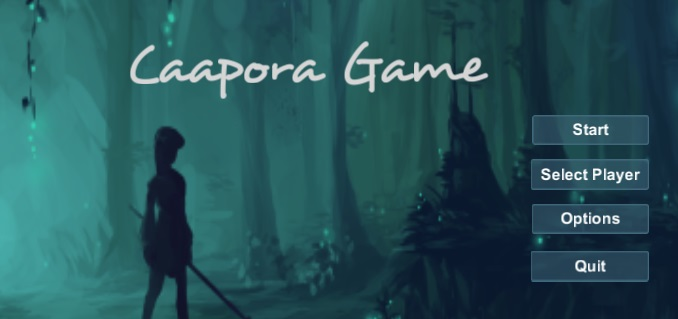
\includegraphics[width=13cm]{figuras/Menu}}
		}{
			\Fonte{Elaborado pelo autor}
		}	
	\end{figure}
	
\subsubsection{Botões}
Para criar os botões no menu foi utilizado um componente chamado UI, ele é um sistema que permite criar interfaces rápida e intuitivas. 

\subsubsection{Título }
Para criar o titulo foi usado um componente do sistema UI, chamado text que permite inserir um texto dentro de uma determinada área. Ele também permite editar alguns detalhes como tipo de fonte, tamanho e cor.

\subsubsection{Imagem de fundo}
Para inserir a imagem de fundo foi preciso adicionar um componente do UI chamado Panel. Ele delimita a área da do jogo, facilitando assim a inserção da imagem de fundo.

\subsection{Jogo}
A cena do jogo foi construída tendo como base o mapa isométrico, que é um cenário mais próximo do 3D. Foi utilizado alguns recursos como: \textit{Tilesets}, \textit{Sprites}, Animação, \textit{Collider} e \textit{Rigidbody}.

A figura 21 mostra o cenário completo.

\begin{figure}[h!]
		\centering
		\Caption{\label{fig:exemplo-1} Cenário do jogo Caapora RPG}	
		\UECEfig{}{
			\fbox{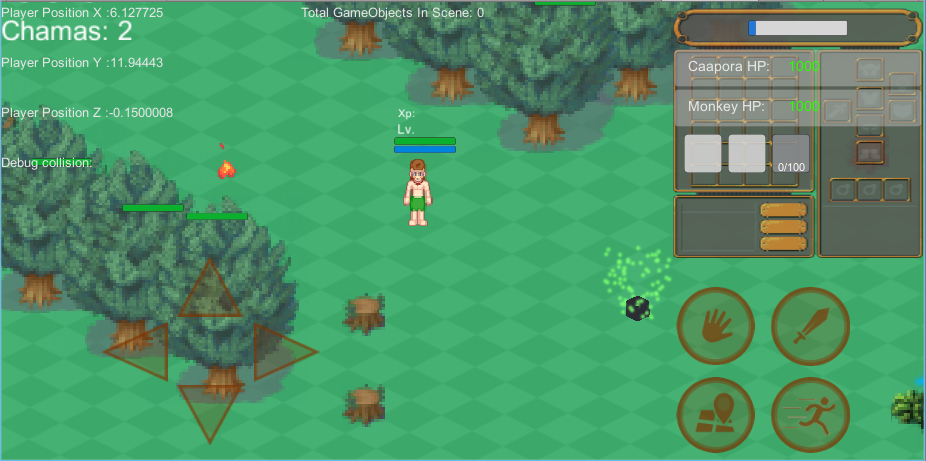
\includegraphics[width=13cm]{figuras/cena}}
		}{
			\Fonte{Elaborado pelo autor}
		}	
	\end{figure}

\subsubsection{Tilesets}
Os \textit{tilesets} são elementos gráficos dentro de uma imagem. Eles possuem tudo o que é preciso para a construção de mapas e são classificados de acordo ao tipo de mapa que será criado, no caso do jogo caipora, foi usado um \textit{tileset} da floresta.

Na figura 22 temos o \textit{tileset} usado no jogo.
\begin{figure}[h!]
		\centering
		\Caption{\label{fig:exemplo-1} Tileset utilizado na criação do cenário}	
		\UECEfig{}{
			\fbox{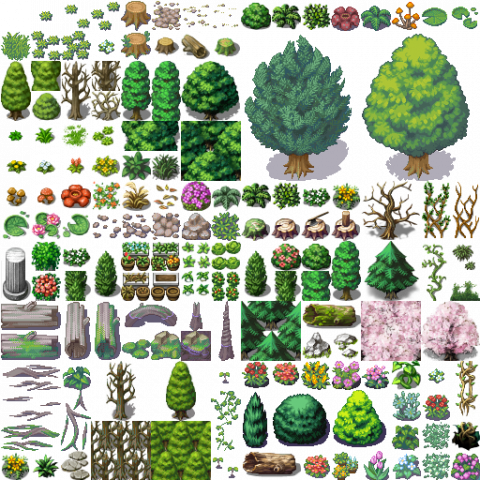
\includegraphics[width=8cm]{figuras/tileset}}
		}{
			\Fonte{\cite{tile}}
		}	
	\end{figure}

\subsubsection{Sprites}
Os \textit{sprites} são elementos gráficos dentro de uma única imagem que tem como objetivo criar animações. Eles foram usados na criação dos personagens e dos animais. 

A figura 23 mostra um dos \textit{sprites} do caipora.

\begin{figure}[h!]
		\centering
		\Caption{\label{fig:exemplo-1} Sprite do caipora correndo}	
		\UECEfig{}{
			\fbox{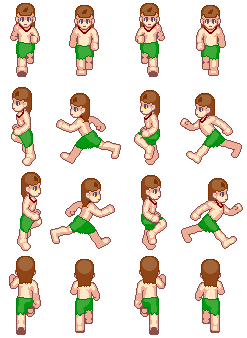
\includegraphics[width=6cm]{figuras/sprite}}
		}{
			\Fonte{Elaborado pelo autor}
		}	
	\end{figure}


\subsubsection{Animação}
A animação, tanto dos personagens quanto dos animais é criado dentro de um componente do Unity chamado Animation. Nele é criado um clipe de animação para cada ação do personagem, onde os \textit{sprites} são inseridos individualmente em uma linha do tempo e é determinada a velocidade que terá a animação.

A figura 24 mostra a criação do clipe de animação “Caapora-left”, onde temos uma sequencia de \textit{sprites} inseridos na linha do tempo.

\begin{figure}[h!]
		\centering
		\Caption{\label{fig:exemplo-1} Componente Animation}	
		\UECEfig{}{
			\fbox{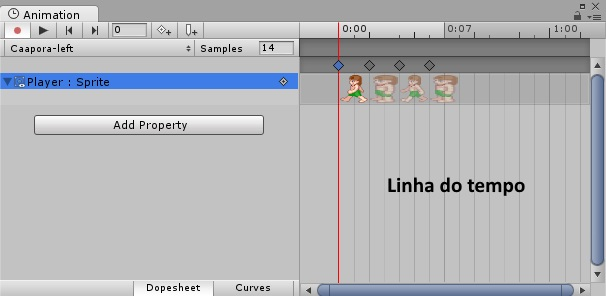
\includegraphics[width=13cm]{figuras/componente}}
		}{
			\Fonte{Elaborado pelo autor}
		}	
	\end{figure}


Após a criação dos clipes de animação, é necessário criar as transições entre eles. Para isso o Unity fornece um componente chamado \textit{Animator}. No \textit{animator}, conforme vemos na figura 25, os clipes de animação são ligados através das transições, que são as setas indo de um clipe para outro, e é criado condições para que haja a transição, ou seja, sempre que houver uma condição dentro do jogo, haverá uma mudança entre os clipes de animação.
	
\pagebreak

\begin{figure}[h!]
		\centering
		\Caption{\label{fig:exemplo-1} Componente Animator}	
		\UECEfig{}{
			\fbox{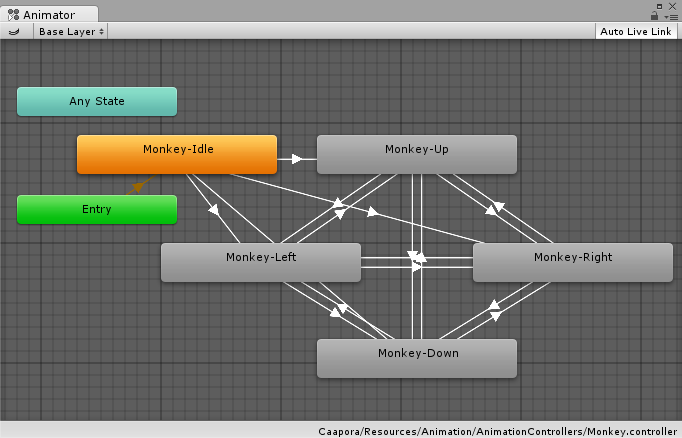
\includegraphics[width=10cm]{figuras/animator}}
		}{
			\Fonte{Elaborado pelo autor}
		}	
	\end{figure}


\subsubsection{Collider}
O colisor é um componente que impede que um objeto transpasse o outro, ele define a forma de um objeto para fins de colisões físicas.

Ele foi utilizado tanto nos personagens quantos nos objetos do cenário afim de evitar que esses objetos não atravessassem os demais.

Na figura 26 temos um tile e o elemento de colisão em volta. As linhas que traçam um retângulo representam o colisor.

	\begin{figure}[h!]
		\centering
		\Caption{\label{fig:exemplo-1} Elemento de colisão em volta de um tile}	
		\UECEfig{}{
			\fbox{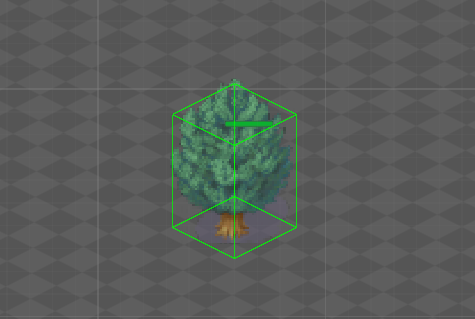
\includegraphics[width=10cm]{figuras/colisor}}
		}{
			\Fonte{Elaborado pelo autor}
		}	
	\end{figure}



\subsubsection{Rigidbody}
O \textit{Rigibody} é um componente que permite um comportamento físico em um determinado objeto. Quando esse componente é anexado ao objeto, automaticamente esse objeto vai responder a gravidade.

A figura 27 mostra o componente \textit{Rigidbody}.
	
	\begin{figure}[h!]
		\centering
		\Caption{\label{fig:exemplo-1} Componente Rigibody}	
		\UECEfig{}{
			\fbox{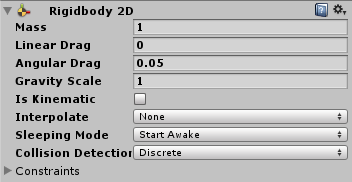
\includegraphics[width=10cm]{figuras/rigi}}
		}{
			\Fonte{Elaborado pelo autor}
		}	
	\end{figure}


\section{Mecanismos}

Nesta seção são apresentados os mecanismos principais que foram desenvolvidos dentro do jogo.

\subsection{Pegar Balde}

 Para implementar este mecanismo foram utilizados os componentes \textit{BoxCollider} do personagem e do elemento balde que ao identificar a colisão um com o outro, permite que o caipora pegue o balde inserindo-o em seu inventário retirando o objeto balde do cenário dando a impressão do objeto ter sido coletado.
 
 O estado do personagem então muda para um estado que identifica ele com o balde e da mesma forma, habilita a animação do caipora para a animação com o balde permitindo que ele colete a água. Na figura 28 é possível visualizar o personagem Caipora com o balde capturado.
 \pagebreak

\begin{figure}[h!]
		\centering
		\Caption{\label{fig:exemplo-1} Caipora com o balde}	
		\UECEfig{}{
			\fbox{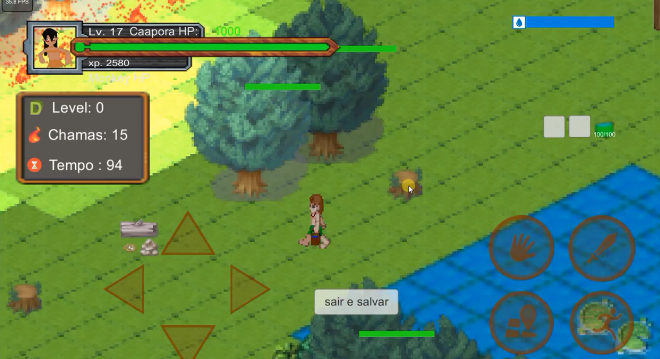
\includegraphics[width=10cm]{figuras/CaiporaComBalde}}
		}{
			\Fonte{Elaborado pelo autor}
		}	
	\end{figure}
	
	
\subsection{Encher o balde e Jogar Água}
Após o Caipora ter pegado o balde ele deverá enche-lo. Para encher o balde o personagem deve ter em seu inventário o balde e ao colidir com o objeto que representa a água um contador é incrementando e o painel de inventário da tela indica visualmente o nível de água que o balde encheu. 

De acordo com a quantidade de água disponível no balde o personagem então poderá lançar no cenário objetos do tipo borrifo de água, que se auto destrói, usando o método Destroy() e o recurso de \textit{Coroutines} do motor de jogos Unity3D, logo após ser lançado.

A figura 29 apresenta o Caipora jogando água nas chamas.

\begin{figure}[h!]
		\centering
		\Caption{\label{fig:exemplo-1} Caipora lançando água nas chamas}	
		\UECEfig{}{
			\fbox{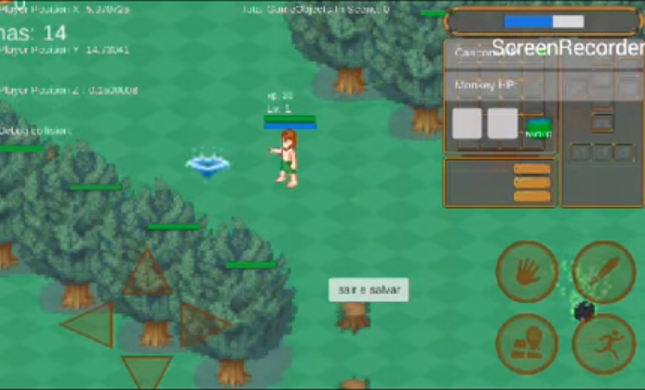
\includegraphics[width=9cm]{figuras/CaiporaJogandoAgua}}
		}{
			\Fonte{Elaborado pelo autor}
		}	
	\end{figure}
	
	
	
\subsection{Chamas}
São objetos que representam as chamas no mundo real e que causam destruição por onde passam, as chamas se multiplicam pelo cenário automaticamente, com o uso de \textit{Coroutines} do motor de jogos Unity3D,  em linha ou em círculos e conforme a dificuldade do jogo eles se espalham mais rapidamente. 

As chamas possuem pontos de danos na classe que as representa que são usados para reduzir os pontos de vida de qualquer personagens vivo no jogo, incluindo árvores. Este comportamento se encontra em todos os seres vivos do jogo que herdam a classe Creature. 

Para destruir este tipo de objetos é necessário que ele utilize o objeto do tipo borrifo de água, que é lançado pelo caipora, causando o efeito de ter apagado as chamas com a água borrifada.

A figura 30 apresenta as chamas se espalhando.

\begin{figure}[h!]
		\centering
		\Caption{\label{fig:exemplo-1} Fogo se alastrando}	
		\UECEfig{}{
			\fbox{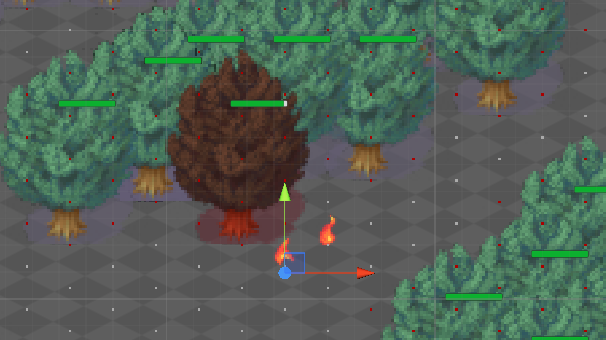
\includegraphics[width=10cm]{figuras/FogoSeAlastrando}}
		}{
			\Fonte{Elaborado pelo autor}
		}	
	\end{figure}
	
	
	
\subsection{Pathfinding}
O algoritmo de busca de melhor caminho (\textit{Pathfinding}) A* foi usado em duas situações no jogo; para personagens NPC (\textit{Non-Player Character}) amigos do personagem principal e para os inimigos que seguem o caipora e seus amigos com o objetivo de ataca-los.  Este recurso faz com que os personagens do jogo se movimentem sozinhos no mapa, melhorando consideravelmente a jogabilidade.


A figura 31 apresenta o personagem NPC \textit{Monkey} seguindo o Caipora com um caminho formado pelo algoritmo A*.

\begin{figure}[h!]
		\centering
		\Caption{\label{fig:exemplo-1} Exemplo de NPC}	
		\UECEfig{}{
			\fbox{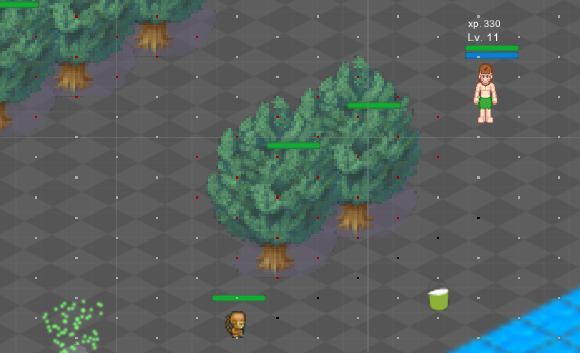
\includegraphics[width=10cm]{figuras/NPC}}
		}{
			\Fonte{Elaborado pelo autor}
		}	
	\end{figure}
	

	\section{Estrutura de Classes}
	A figura 32 apresenta a estrutura de Classes dos Personagens utilizada para o desenvolvimento do jogo.
	
	\begin{figure}[h!]
		\centering
		\Caption{\label{fig:exemplo-1} Estrutura de Classes de Personagens }	
		\UECEfig{}{
			\fbox{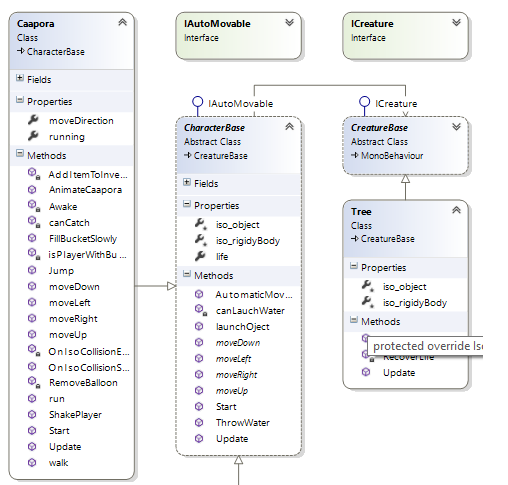
\includegraphics[width=15cm]{figuras/DiagramaClassesPersonagens}}
		}{
			\Fonte{Elaborado pelo autor}
		}	
	\end{figure}
	\pagebreak
	
\subsection{GameManager}
Está classe é responsável por gerenciador todo o ciclo de vida do jogo para isso ela  utiliza o padrão de projeto \textit{Singleton} que garante apenas uma instancia para um objeto durante toda a execução do jogo. Ela que implementa a maior parte da regra de negócio do jogo incluindo condições de vitórias e o fim de jogo.

\pagebreak

\subsection{Enemy}
Classe que representa os estados e comportamentos dos inimigos no jogo.

\subsection{NPC}
Personagens deste tipo implementam o algorítimo de \textit{pathfinding}  permitindo que movimentem-se sozinhos no jogo, possuindo uma inteligência artificial. Utiliza os métodos da classe \textit{Pathfinding} para personagens que perseguem o Caipora, é utilizando tanto amigos quanto em inimigos.

A figura 33 apresenta a estrutura de Classes dos NPCs utilizada para o desenvolvimento do jogo.

	\begin{figure}[h!]
		\centering
		\Caption{\label{fig:exemplo-1} Estrutura de Classes de NPC's }	
		\UECEfig{}{
			\fbox{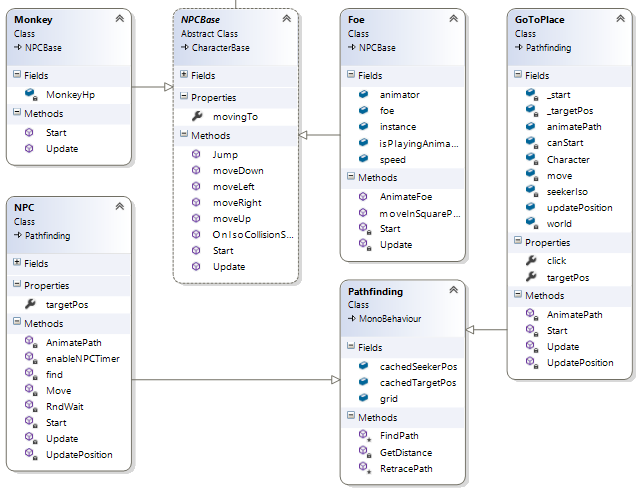
\includegraphics[width=15cm]{figuras/DiagramaClassesNpc}}
		}{
			\Fonte{Elaborado pelo autor}
		}	
	\end{figure}

\subsection{Inventory}
Esta classe tem por finalidade armazenar os objetos coletados pelo personagem principal e exibir suas características. Como exemplo temos o balde que no início do jogo o caipora tem que pegá-lo e enche-lo para apagar as chamas que estão queimando as árvores.


\subsection{Tree}
Esta classe representa as árvores no cenário e possui características herdadas da classe abstrata CreatureBase, possuindo assim pontos de vida e ataque podendo  morrer ao sofrer danos.


\subsection{Water}
Classe que representa a água no cenário, ao colidir com o fogo apaga-o. Ao colidir com o Caipora com o balde aumenta a quantidade de água no balde.


\subsection{Fire}
Classe que representa um fogo no \textit{game}, possui pontos de danos que são utilizados quando objetos do tipo seres vivos colidem com ele reduzindo seus pontos de vida.


\subsection{SpreadFire}
Classe que automatiza a expansão do fogo pelo cenário, extraindo as instâncias do \textit{Object Pool} e inserindo no mapa tanto em linha quanto em círculos.

\section{Funcionamento do jogo}
A aplicação do Caapora RPG se inicia no menu principal, onde o jogador pode iniciar o jogo, escolher um personagem, alterar configurações e sair do jogo como mostra a figura 34.

\pagebreak
\begin{figure}[h!]
		\centering
		\Caption{\label{fig:exemplo-1} Menu Principal}	
		\UECEfig{}{
			\fbox{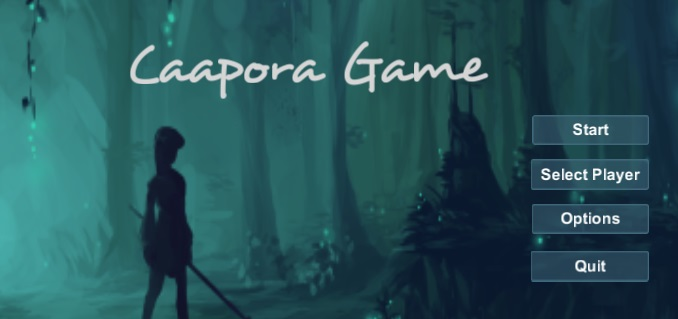
\includegraphics[width=13cm]{figuras/Menu}}
		}{
			\Fonte{Elaborado pelo autor}
		}	
	\end{figure}

Jogar: Ao selecionar a opção jogar, é apresentado ao jogador a tela do tutorial, onde terá uma breve descrição do que o jogador deverá fazer durante o jogo.

Personagem: Ao selecionar a opção personagem, o jogador será direcionado para tela onde ele poderá selecionar o Caipora ou o Curupira para jogar.

Opções: Ao selecionar o botão opções, o jogador poderá alterar algumas configurações como tirar a musica de fundo.

Sair: Ao selecionar o botão sair o jogador fecha o jogo.

Ao iniciar o jogo, a missão do jogador é apagar o fogo que está destruindo a mata, para isso ele deverá pegar um balde que está próximo ao rio, como mostra a figura 35.

\pagebreak
\begin{figure}[h!]
		\centering
		\Caption{\label{fig:exemplo-1} Jogador próximo ao balde.}	
		\UECEfig{}{
			\fbox{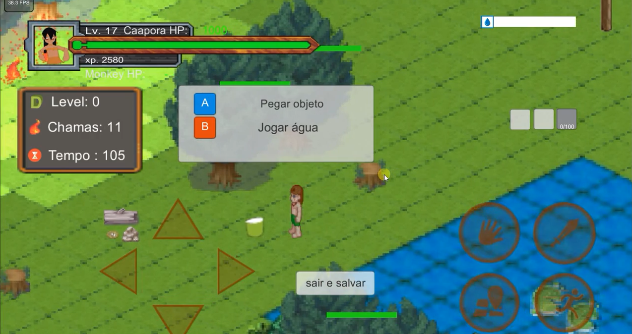
\includegraphics[width=13cm]{figuras/CaiporaPegandoBalde}}
		}{
			\Fonte{Elaborado pelo autor}
		}	
	\end{figure}

Ao pegar o balde o jogador deverá se dirigir até o rio, onde ao entrar em contato com o rio o balde encherá automaticamente. Na figura 36 temos o caipora enchendo o balde.

\begin{figure}[h!]
		\centering
		\Caption{\label{fig:exemplo-1} Jogador próximo ao rio.}	
		\UECEfig{}{
			\fbox{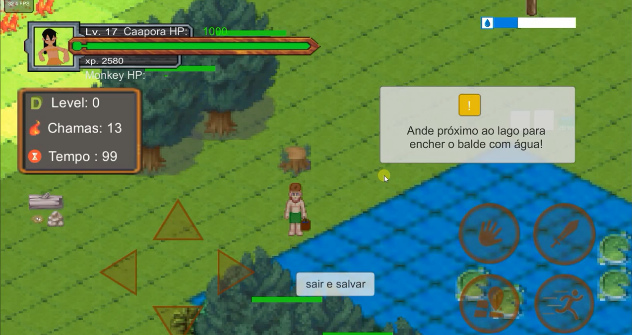
\includegraphics[width=13cm]{figuras/EnchendoBalde}}
		}{
			\Fonte{Elaborado pelo autor}
		}	
	\end{figure}

Com isso o jogador deverá procurar os lugares na floresta onde a mata esta em chamas. Dentro do jogo, o jogador terá um recurso que permitirá que ele visualize todo o mapa, sabendo assim onde se encontra o fogo. Na figura 37 temos o mapa completo do jogo.

\pagebreak
\begin{figure}[h!]
		\centering
		\Caption{\label{fig:exemplo-1} Mapa completo do jogo.}	
		\UECEfig{}{
			\fbox{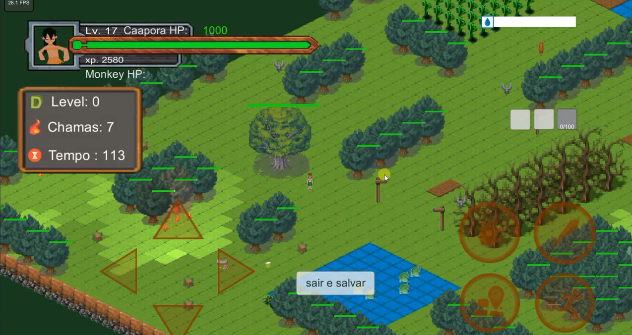
\includegraphics[width=13cm]{figuras/MapaCompleto}}
		}{
			\Fonte{Elaborado pelo autor}
		}	
	\end{figure}

Após localizar o local onde a mata esta pegando fogo, o jogador deverá lançar a água. A missão terminá quando todo o fogo na floresta for apagado. Os detalhes da missão estão descritos no \textit{Game Design Document} que esta no Apêndice.
